\section{Chain Unit}
\label{sec:chain}

\emph{Chain} unit is another type of input to BGPmon.  \emph{Chain} unit  provide XML messages that include BGP messages from other BGPmon instances.  However, \emph{Chain} unit can be a type of output source: it is a client to BGPmon that receives XML messages.    \emph{Chain} unit include two types of chain setups: \emph{Chain IN} and \emph{Chain OUT} units. First, \emph{Chain IN} is setup of BGPmon application that sends XML messages to BGPmon test instance. Second, \emph{Chain OUT} is setup of BGPmon application that receives XML messages from BGPmon test instance. Thus, \emph{Chain IN} and \emph{Chain OUT} units are designed to create a mesh network of BGPmons. Overall, \emph{Chain} unit is designed to archive following goals in a BGPmon Test Framework:
\begin{itemize}
\item{Test BGPmon instance to scale out through chaining other BGPmons.}
\item{Receive and send XML messages: this verifies that BGPmon is able to receive XML messages from connected chain instance and forward XML messages to other chain instaces.}
\end{itemize}


\subsection{IPv4 Chain IN Unit}

\begin{figure}
\centering
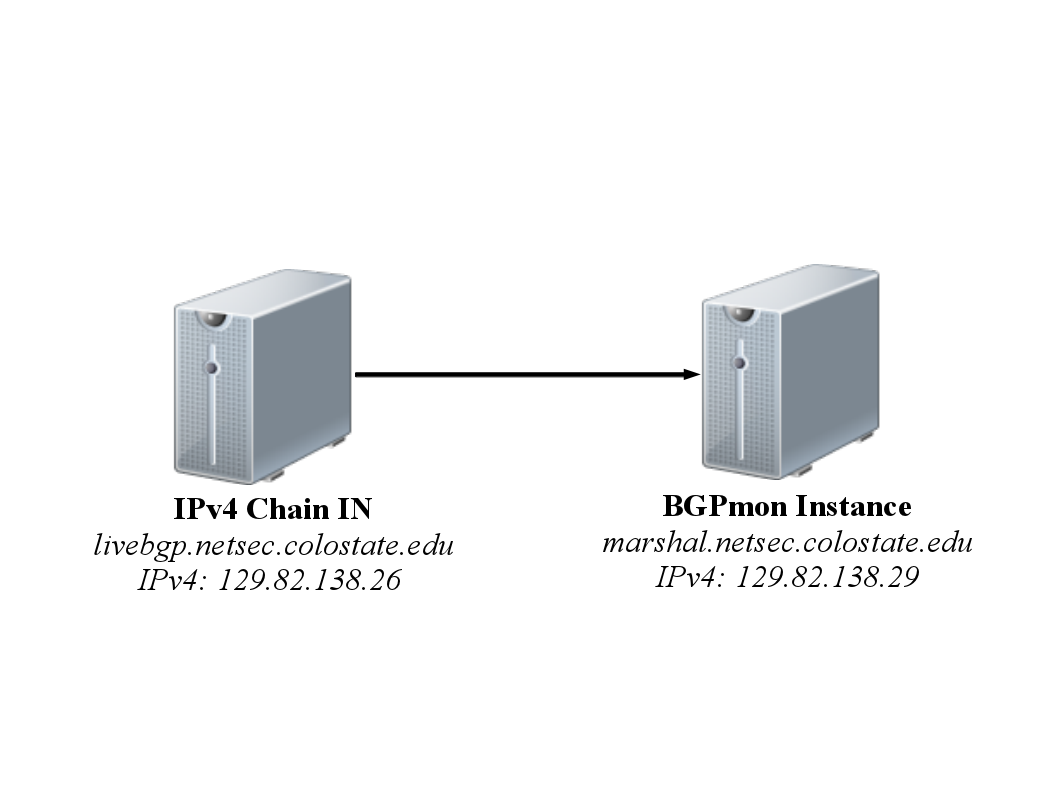
\includegraphics[scale=0.30]{figs/ipv4-chain-in.png}
\caption{An overview of Chain IN Unit.}
\label{chainin}
\end{figure}

Figure \ref{chainin} shows test unit design: it has \emph{IPv4 Chain IN} unit on the left  and BGPmon testing instance on the right.  \emph{IPv4 Chain IN} unit is installed on \emph{livebgp.netsec.colostate.edu} with \emph{129.82.138.26} IPv4 address. \emph{IPv4 Chain IN} unit provide stream of XML update messages on port \emph{50001} and stream of XML table messages on port \emph{50002}. BGPmon test instance is configured on \emph{marshal.netsec.colostate.edu} with \emph{129.82.138.29} IPv4 address.

\subsubsection{IPv4 Chain IN Unit Launch}

To start IPv4 Chain IN unit:

\begin{enumerate}
\item{Login to \emph{marshal.netsec.colostate.edu}}
  \begin{enumerate}
  \item{Make sure that BGPmon process is up and running. If not, see Section \ref{sec:essentials}.}
  \item{Telnet to \emph{localhost} port \emph{50000} to Command Line Interface.}
  \item{In \emph{configuration mode}, launch:}
    \begin{verbatim}
     marshal# chain 129.82.138.26 enable
    \end{verbatim}
  \end{enumerate}
\item{IPv4 Chain IN instance that run on \emph{livebgp.netsec.colostate.edu} does not require any configuration, its ready for use.}
\end{enumerate}

\subsubsection{IPv4 Chain IN Unit Configuration}

In order to start providing XML messages,  \emph{IPv4 Chain IN} unit require to have at least one of three inputs of BGP messages. User if free to configure \emph{Peer}, \emph{MRT} or another \emph{IPv4 Chain} unit.

\subsubsection{BGPmon Test Instance Configuration}

In order to run \emph{IPv4 Chain IN} unit, user of framework need to enable chain  at BGPmon  test instance. To enable chain session, log in to \emph{marshal.netsec.colostate.edu} and ensure that BGPmon process is up and running.  

To enable chain from \emph{IPv4 Chain IN} unit to  BGPmon test instance, run following command in Command Line Interface (CLI):

\begin{verbatim}
marshal# chain 129.82.138.26 enable
\end{verbatim}

At this point, BGPmon test instance opens two opens two TCP connections to \emph{IPv4 Chain IN} unit and receives stream of XML messages. 

To disable chain to \emph{IPv4 Chain IN} unit, run:

\begin{verbatim}
marshal# chain 129.82.138.26 disable
\end{verbatim}

\subsubsection{Result reporting}

In order to verify if configuration was successfully enabled, run following command in CLI on BGPmon test instance:

\begin{verbatim}
marshal>show chains
\end{verbatim}

This commands lists chain session that was enabled. In case of successfully enabled chain session,  CLI will show following report:

\begin{verbatim}
marshal>show chains
ID	address		uport	rport	retry	status
0	129.82.138.26	50001	50002 60   enabled
\end{verbatim}







\subsection{IPv4 Chain OUT Unit}

\begin{figure}
\centering
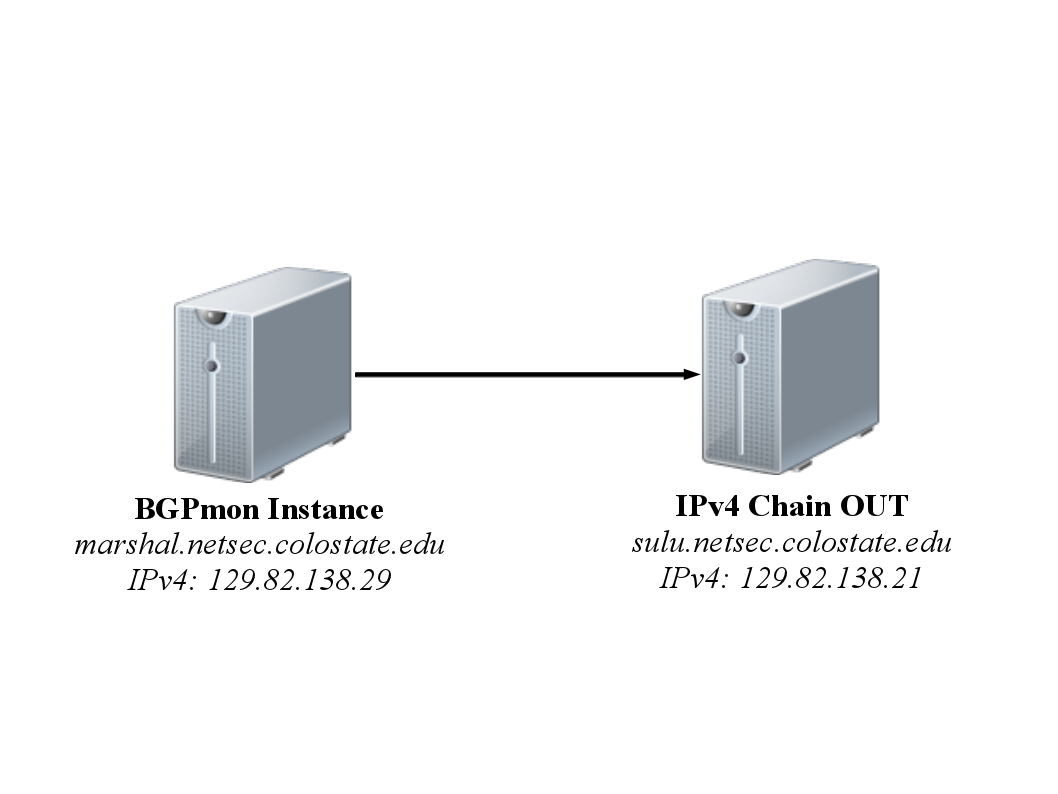
\includegraphics[scale=0.30]{figs/ipv4-chain-out.png}
\caption{An overview of Chain OUT Unit.}
\label{chainout}
\end{figure}

Figure \ref{chainout} shows test unit design: it has \emph{IPv4 Chain OUT} on the fight unit and BGPmon testing instance on the left.  \emph{IPv4 Chain OUT} unit is installed on \emph{sulu.netsec.colostate.edu} with \emph{129.82.138.21} IPv4 address.  BGPmon test instance is configured on \emph{marshal.netsec.colostate.edu} with \emph{129.82.138.29} IPv4 address. In this design BGPmon test unit provide stream of XML update messages on port \emph{50001} and stream of XML table messages on port \emph{50002}.

\subsubsection{IPv4 Chain OUT Unit Configuration}

In order to run \emph{IPv4 Chain OUT} unit, user of framework need to enable chain  at \emph{IPv4 Chain OUT} unit. To enable chain session, log in to \emph{sulu.netsec.colostate.edu} and ensure that BGPmon process is up and running.  

To enable chain from  BGPmon test instance to \emph{IPv4 Chain OUT} unit, run following command in Command Line Interface (CLI):

\begin{verbatim}
marshal# chain 129.82.138.29 enable
\end{verbatim}

At this point, \emph{IPv4 Chain OUT} unit opens two opens two TCP connections to BGPmon test unit and receives stream of XML messages. 

To disable chain to BGPmon test instance, run:

\begin{verbatim}
marshal# chain 129.82.138.29 disable
\end{verbatim}


\subsubsection{BGPmon Test Instance Configuration}

To start sending XML messages,  BGPmon test instance require to have at least one of three inputs of BGP messages. User if free to choose any available like \emph{Peer}, \emph{MRT} or another \emph{IPv4 Chain} unit.



\subsubsection{Result reporting}

In order to verify if configuration was successfully enabled, run following command in CLI on \emph{IPv4 Chain OUT} unit:

\begin{verbatim}
marshal>show chains
\end{verbatim}

This commands lists chain session that was enabled. In case of successfully enabled chain session to BGPmon test unit,  CLI  shows following report:

\begin{verbatim}
marshal>show chains
ID	address		uport	rport	retry	status
0	129.82.138.29	50001	50002 60   enabled
\end{verbatim}



%Test unit above verifies that Test BGPmon Instance is able to establish and receive XML data from BGPmon Source Instance.   In order to verify that Testing BGPmon Instance can provide XML feed to the clients,  run \emph{WebStat Client Test Unit} that described in Section \ref{sec:webclient}

%To ensure that \emph{Testing BGPmon} is able to receive and process XML stream, user need to telnet to \emph{marshal.netsec.colostate.edu} port \emph{50001} to receive stream of update messages in XML format. To accomplish this, run:

%\begin{verbatim}
%$ telnet marshal.netsec.colostate.edu 50001
%\end{verbatim}

%To test RIB-IN XML stream, telnet to \emph{marshal.netsec.colostate.edu} port \emph{50002}: 
%\begin{verbatim}
%$ telnet marshal.netsec.colostate.edu 50002
%\end{verbatim}
